% =====================================================================
%  ANCHOR — A1 BETTER POSTER (landscape)
%
%  Three-column layout:
%    Left   (~22%, cream):   title, authors, BACKGROUND / APPROACH /
%                            OUTCOMES / LINEAGE.
%    Centre (~56%, flat dark teal): logos, big takeaway, subline,
%                            funding footer.
%    Right  (~22%, cream):   graphical-abstract slot, WHAT INDUSTRY
%                            GETS, READ MORE + QR.
%
%  Compile with XeLaTeX:
%      latexmk better-poster.tex
% =====================================================================

\documentclass{article}

\usepackage[paperwidth=841mm, paperheight=594mm,
            margin=0pt, noheadfoot]{geometry}
\usepackage{fontspec}
\usepackage{xcolor}
\usepackage{graphicx}
\usepackage{tikz}
\usetikzlibrary{shadows}
\usepackage[absolute, overlay]{textpos}
\usepackage{ragged2e}
\usepackage{microtype}
\usepackage[hidelinks]{hyperref}
\usepackage{qrcode}

% Fonts
\setmainfont{Open Sans}
\newfontfamily\headingfont{Montserrat}
\newfontfamily\titlefont{Montserrat ExtraBold}
\newfontfamily\bigfont{Montserrat Black}
%\newfontfamily\monofont{Menlo}
\setmonofont{Consolas}

% Colour palette — Anchor is the warm-orange sibling of the yellow PhD posters
\definecolor{paneltext}{HTML}{1B1B1B}
\definecolor{panelbg}{HTML}{F2EFE8}     % warm cream for side panels
\definecolor{panelmuted}{HTML}{6E6E6E}  % muted body grey
\definecolor{centerbg}{HTML}{0F3438}    % flat dark teal centre band
\definecolor{centertext}{HTML}{FFFFFF}
\definecolor{centermuted}{HTML}{B8C9CB} % muted text on dark teal
\definecolor{accent}{HTML}{FF8E2B}      % warm orange highlight
\definecolor{slotborder}{HTML}{C9C2B4}  % dashed border for the figure slot

% TextPos in mm
\setlength{\TPHorizModule}{1mm}
\setlength{\TPVertModule}{1mm}
\textblockorigin{0mm}{0mm}

\graphicspath{{../assets/}{assets/}{screenshots/}{figures/}{generated/}{./}}

\pagestyle{empty}
\setlength{\parindent}{0pt}
\setlength{\parskip}{0.55\baselineskip}
\linespread{1.18}

% Column geometry (mm). Landscape A1: 22/56/22 split of 841 mm width.
\newcommand{\leftColW}{185}
\newcommand{\centerColX}{185}
\newcommand{\centerColW}{471}
\newcommand{\rightColX}{656}
\newcommand{\rightColW}{185}
\newcommand{\panelPad}{14}
\newcommand{\barH}{55}         % black title bar across the top (mm)
\newcommand{\contentTop}{60}   % where content starts below the bar

% Side-panel section heading
\newcommand{\panelhead}[1]{%
  \par\addvspace{5mm}%
  {\headingfont\bfseries\fontsize{14pt}{17pt}\selectfont
   \MakeUppercase{#1}\par}%
  \nopagebreak\vspace{1mm}%
  \textcolor{accent}{\rule{32mm}{1.5pt}}\par
  \vspace{1.5mm}%
}

% Highlight a phrase inside the big takeaway
\newcommand{\hl}[1]{\textcolor{accent}{#1}}

% Arrow that renders in any font (Open Sans Regular lacks U+2192).
\newcommand{\arr}{\ensuremath{\rightarrow}}

\begin{document}

% ---------------------------------------------------------------------
%  BACKGROUND PANELS
% ---------------------------------------------------------------------
\begin{tikzpicture}[remember picture, overlay]
  % --- BLACK TITLE BAR across the full width at the very top ---------
  % Sub-hero: gives identity at a glance, but the centre takeaway
  % below is still the visual heavyweight (better-poster ideology).
  \fill[black]
     (current page.north west)
     rectangle
     ([yshift=-\barH mm]current page.north east);

  % --- Left & right cream panels (start below the bar) ---------------
  \fill[panelbg]
     ([yshift=-\barH mm]current page.north west)
     rectangle
     ([xshift=\leftColW mm]current page.south west);
  \fill[panelbg]
     ([xshift=\rightColX mm, yshift=-\barH mm]current page.north west)
     rectangle
     (current page.south east);

  % --- Centre band: cruise_grad.png (starts below the bar) -----------
  % Image is 2250×4000 px; new band aspect = 471/(594-55) = 471/539
  % ≈ 0.874 → keep a 2250×2575 strip. Anchor to the bottom of the
  % source so the darkest sea lands at the bottom of the column where
  % the funding line sits.
  \node[anchor=north west, inner sep=0pt]
     at ([xshift=\centerColX mm, yshift=-\barH mm]current page.north west)
     {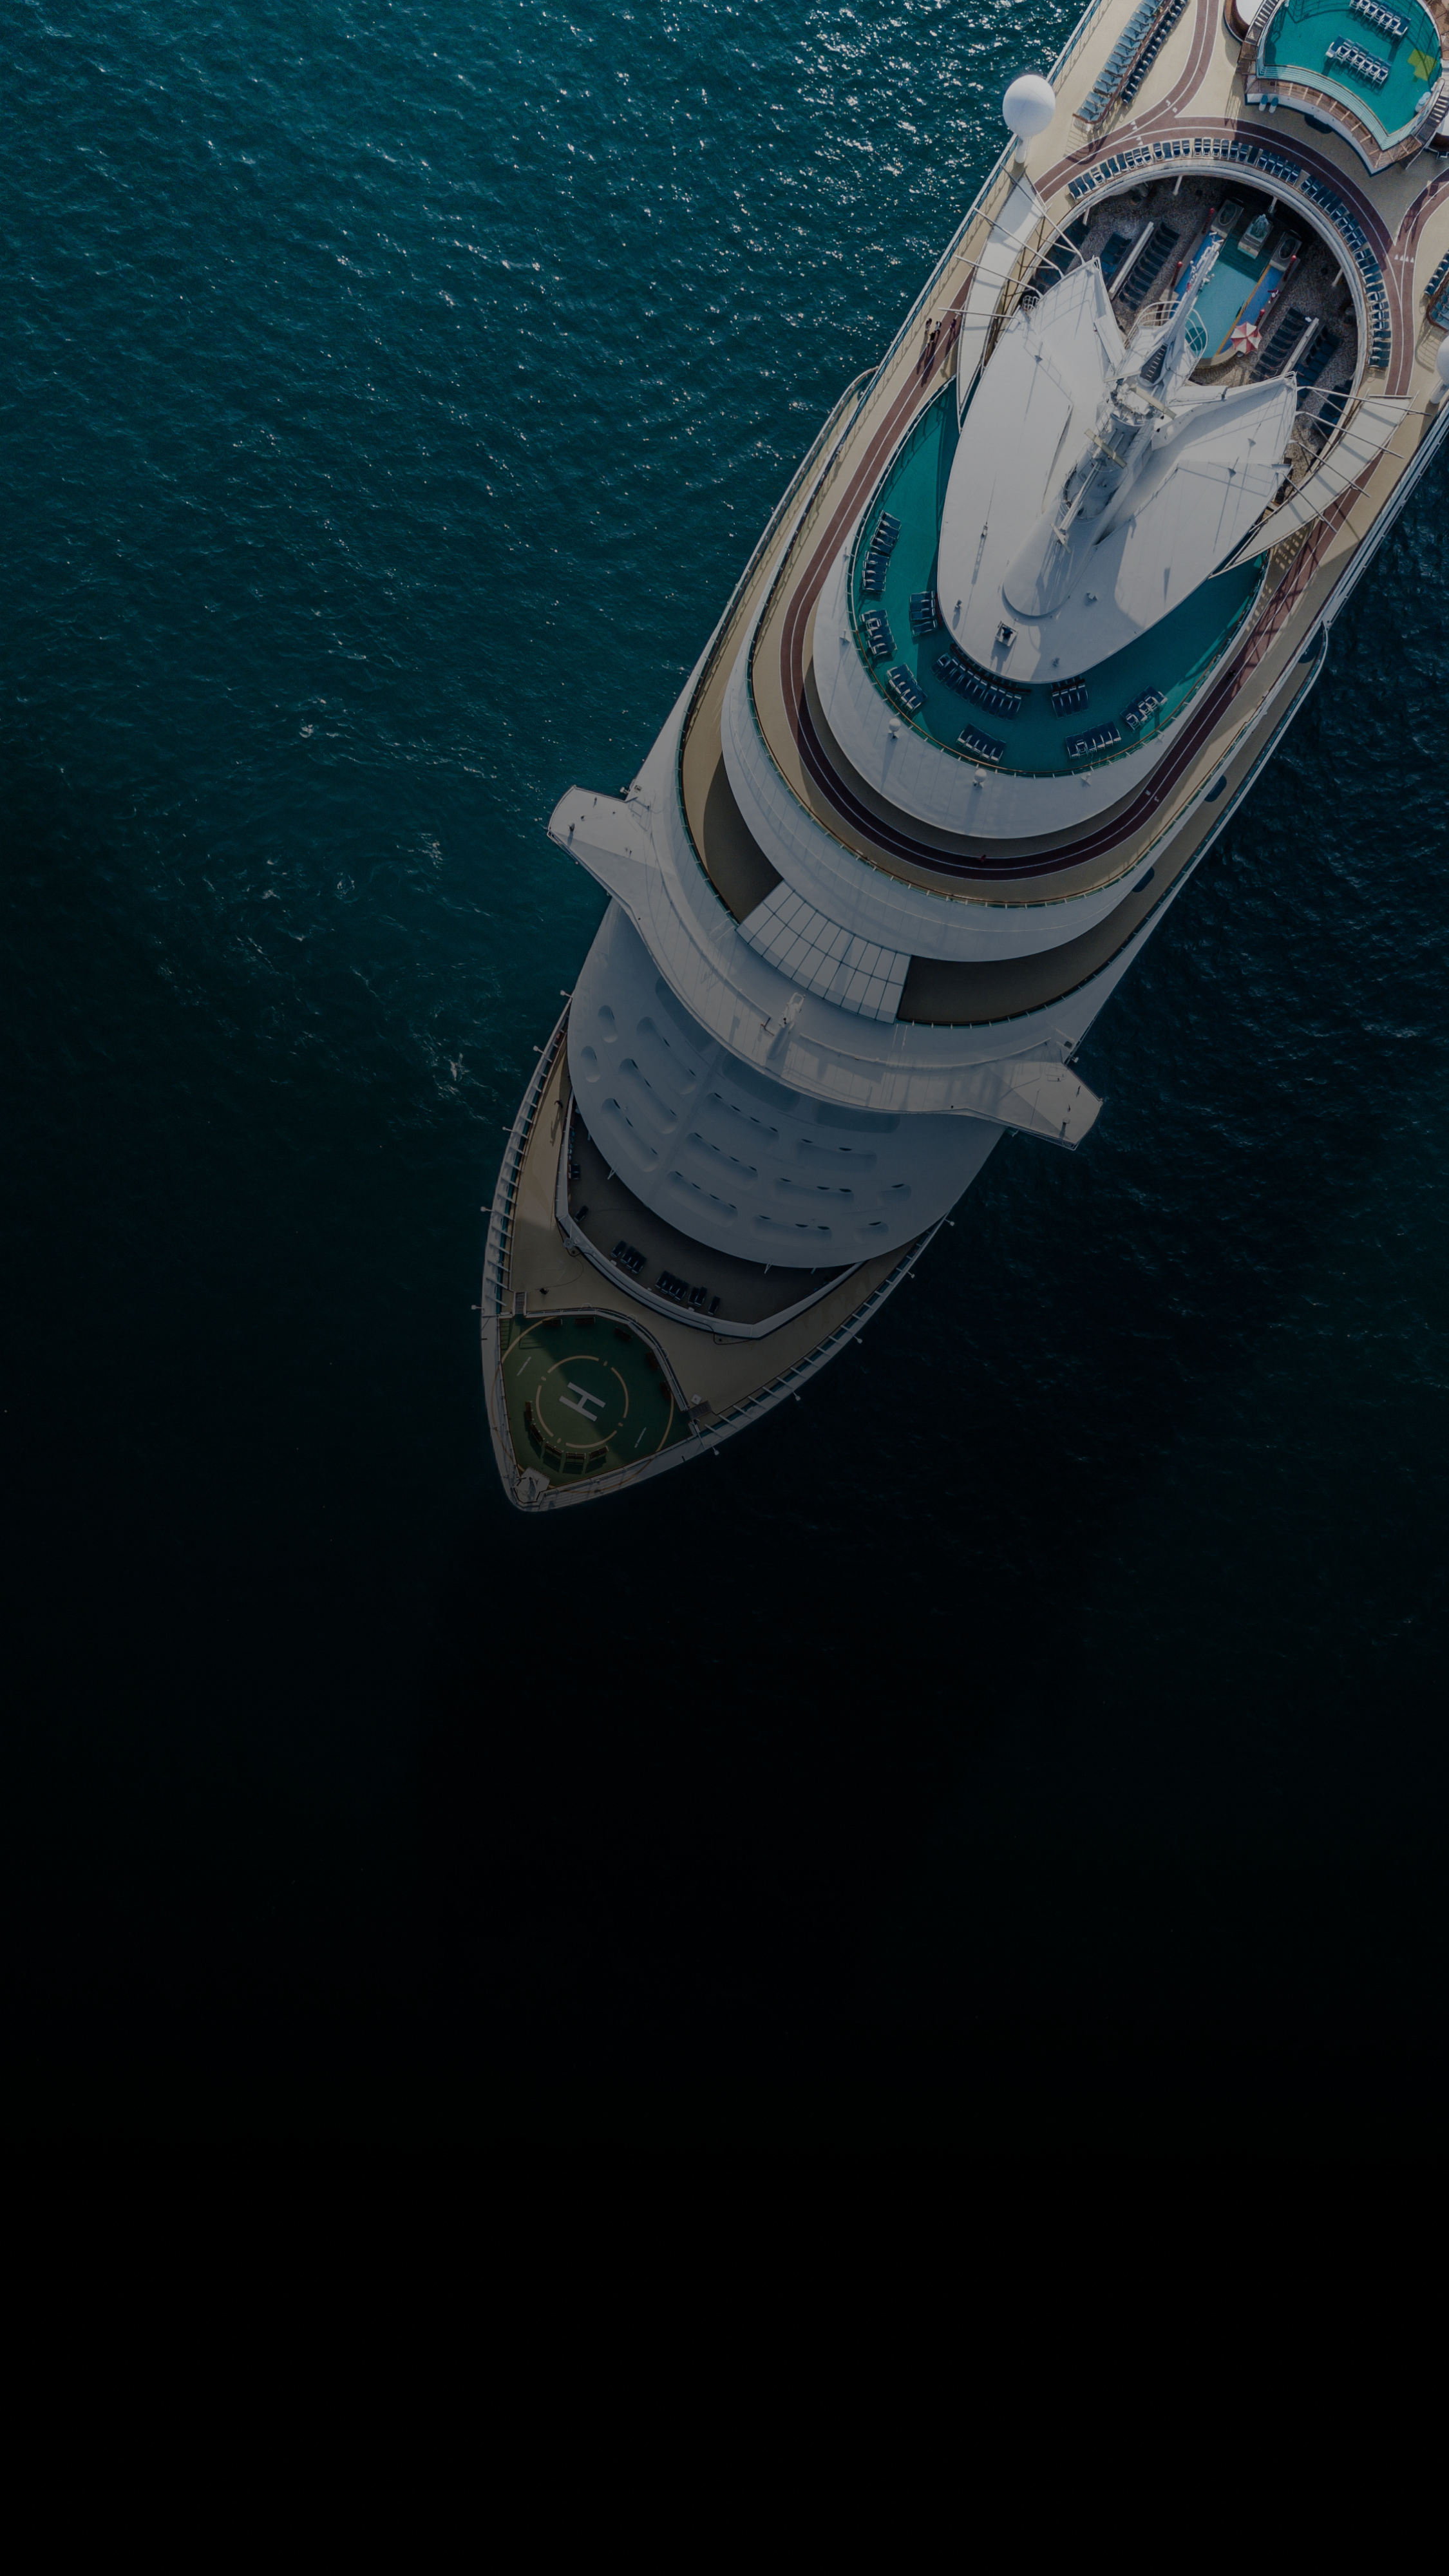
\includegraphics[width=\centerColW mm,
                       viewport=0 0 2250 2575, clip]{cruise_grad.png}};
\end{tikzpicture}

% ---------------------------------------------------------------------
%  TOP BAR — Anchor mark + wordmark + tagline / Novia logo
% ---------------------------------------------------------------------
% Left side of the bar: logo mark + wordmark + tagline.
\begin{textblock}{600}(20,8)
  \color{centertext}
  \begin{minipage}[c]{\linewidth}
    
\includegraphics[height=36mm]{anchor-white.pdf}\hspace{6mm}%
    \raisebox{6mm}{%
      \begin{minipage}[b]{0.78\linewidth}
        {\headingfont\bfseries\fontsize{52pt}{52pt}\selectfont Anchor\par}
        \vspace{2mm}
        {\headingfont\fontsize{14pt}{17pt}\selectfont
         % Two MCP tools. Datasheets in, grounded answers out.
         Datasheets in. Page-grounded answers out.\par}
      \end{minipage}}%
  \end{minipage}
\end{textblock}

% Right side of the bar: Novia logo (white, on black). Anchor poster
% uses Novia only — no ÅA logo on this one.
\begin{textblock}{160}(665,17)
  \color{centertext}\hfill
  
\includegraphics[height=30mm]{logoinvinternwhite.pdf}\hfill\strut
\end{textblock}

% ---------------------------------------------------------------------
%  LEFT COLUMN — authors + paper-style content
% ---------------------------------------------------------------------
\begin{textblock}{157}(14,\contentTop)          % 185 - 2*14 = 157 mm wide
  \color{paneltext}\fontsize{11pt}{15pt}\selectfont\RaggedRight

  {\fontsize{9.5pt}{13pt}\selectfont
   \textbf{Christoffer Björkskog} · christoffer.bjorkskog@novia.fi\par
   \vspace{1mm}
   \textbf{Lamin Jatta} · lamin.jatta@novia.fi\par
   Maritime Technology, Novia University of Applied Sciences\par
   \vspace{1mm}
   \textbf{Supervisors:} Andreas Lundell (ÅAU),
   Johan Westö (Novia UAS), Mikael Manngård (Novia UAS).\par}

  \panelhead{Problem}
  Engineers still copy values from datasheets, product leaflets, P\&ID drawings, and
  control-system manuals into spreadsheets and simulation models by hand.
  % Free-text RAG (normal LLMs answers) hides the citation; and where the numbers came from.
  Normal chat answers hide where numbers came from.
  One wrong pressure, temperature, or dimension can travel into a calculation with no
  route back to the source page
  % One mis-transcribed parameter lands in a safety calculation with no way back to the source page.

  % \panelhead{Architecture}
  % Two MCP services over three folders on disk:
  % \begin{itemize}\setlength{\itemsep}{1.5pt}\setlength{\parsep}{1pt}\setlength{\leftmargin}{4mm}
  %   \item \textbf{DOCS} — bronze (raw PDFs) \arr{} silver (page
  %     layout + text) \arr{} gold (regions with page + bbox).
  %   \item \textbf{CANVASES} — one folder per canvas. Share like a file.
  %   \item \textbf{SESSION} — live state in memory; the same JSON
  %     drives every UI.
  % \end{itemize}
  % \texttt{IngestService} turns PDFs into the gold layer.
  % \texttt{WorkspaceService} records every canvas action as a versioned
  % event. Both speak MCP, HTTP, and SSE.
  \panelhead{What Anchor Does}
  Anchor makes document evidence visible and reusable:
  \begin{itemize}\setlength{\itemsep}{1.5pt}\setlength{\parsep}{1pt}\setlength{\leftmargin}{4mm}
    \item Drop technical PDFs into a shared engineering workspace.
    \item Convert pages into text, images, tables, figures, and semantic regions.
    \item Ask an agent for specs, operating limits, tables, or facts.
    \item Place grounded cards on the canvas with source links.
    \item Jump from a canvas answer back to the exact PDF page and region.
    \item Keep document evidence separate from FMU wiring so engineers stay in control.
  \end{itemize}

  \panelhead{How It Works}
  \begin{itemize}\setlength{\itemsep}{1.5pt}\setlength{\parsep}{1pt}\setlength{\leftmargin}{4mm}
    % Bronze \rarr{} Silver \rarr{} Gold \rarr{} Canvas
    % \textbf{Bronze} $\rightarrow$ \textbf{Silver} $\rightarrow$ \textbf{Gold} $\rightarrow$ \textbf{Canvas}
    %Bronze $\rightarrow$ Silver $\rightarrow$ Gold $\rightarrow$ Canvas
    \item Bronze $\rightarrow$ Silver $\rightarrow$ Gold $\rightarrow$ Canvas
    \par Bronze:
    Raw uploaded PDFs.
    \par Silver:
    Page markdown, page images, outlines, tables, figures, and document index.
    \par Gold:
    Semantic regions such as tables, charts, diagrams, captions, text blocks, and
    spec blocks. Each region can carry page and bbox provenance.
    \par Canvas:
    React Flow workspace with document cards, facts, spec tables, images, FMUs,
    plots, notes, and visible source/evidence edges.
  \end{itemize}


  \panelhead{What v0.1 ships}
  \begin{itemize}\setlength{\itemsep}{1.5pt}\setlength{\parsep}{1pt}\setlength{\leftmargin}{4mm}
    % \item \textbf{17 MCP commands} — 6 ingest, 11 canvas. Claude Code,
    % Cursor, or your own agent drives the same data.
    % \item \textbf{Web UI in the same backend.} Drop a PDF; ingest
    %   progress streams to every browser tab and agent.
    % \item \textbf{$\sim$100\,ms multi-client sync} between agents
    %   and browsers.
    \item Upload PDFs and run the medallion document pipeline.
    \item Inspect bronze, silver, and gold status in the right rail.
    \item Ask grounded questions over documents on the canvas.
    \item Create fact cards, image crops, and spec/table nodes from document evidence.
    \item Keep source chips on answers and table rows.
    \item Click sources to reopen the PDF page with highlights.
    \item Store conversations and canvas evidence for later review.
  \end{itemize}

  \panelhead{Boundary}
  % Automatic document-to-FMU wiring is fully end-to-end.
  FMU upload, inspect, and simulation routes exist, and FMU nodes are part
  of the canvas. Automatic document-to-FMU wiring is still manual and
  experimental; engineers review values before wiring them into simulations.

  \vfill
  {\color{panelmuted}\fontsize{8.5pt}{11pt}\selectfont
   Novia University of Applied Sciences\par}
\end{textblock}

% ---------------------------------------------------------------------
%  CENTRE COLUMN — big takeaway, flow strip, footer
%  (Project identity + logos now live in the top bar.)
% ---------------------------------------------------------------------

% BIG TAKEAWAY — sits over the dark sea below the cruise ship deck
\begin{textblock}{443}(199,205)
  \color{centertext}\centering
  {\bigfont\fontsize{72pt}{86pt}\selectfont
   Every spec your agent quotes\\
   points back to the\\
   \hl{page it came from}.\par}
  \vspace{10mm}
  {\headingfont\fontsize{22pt}{28pt}\selectfont
   Datasheet \arr{} canvas \arr{} simulation.\\
   \emph{Provenance built in.}\par}
\end{textblock}

% --- ARCHITECTURE DIAGRAM on the dark sea, below the takeaway --------
% Hand-drawn-style figure from paperx/figures/architecture.png.
% Black-on-black aesthetic merges with the dark sea backdrop. Centred
% horizontally in the centre column.
\begin{textblock}{443}(199,355)
  \centering
  % 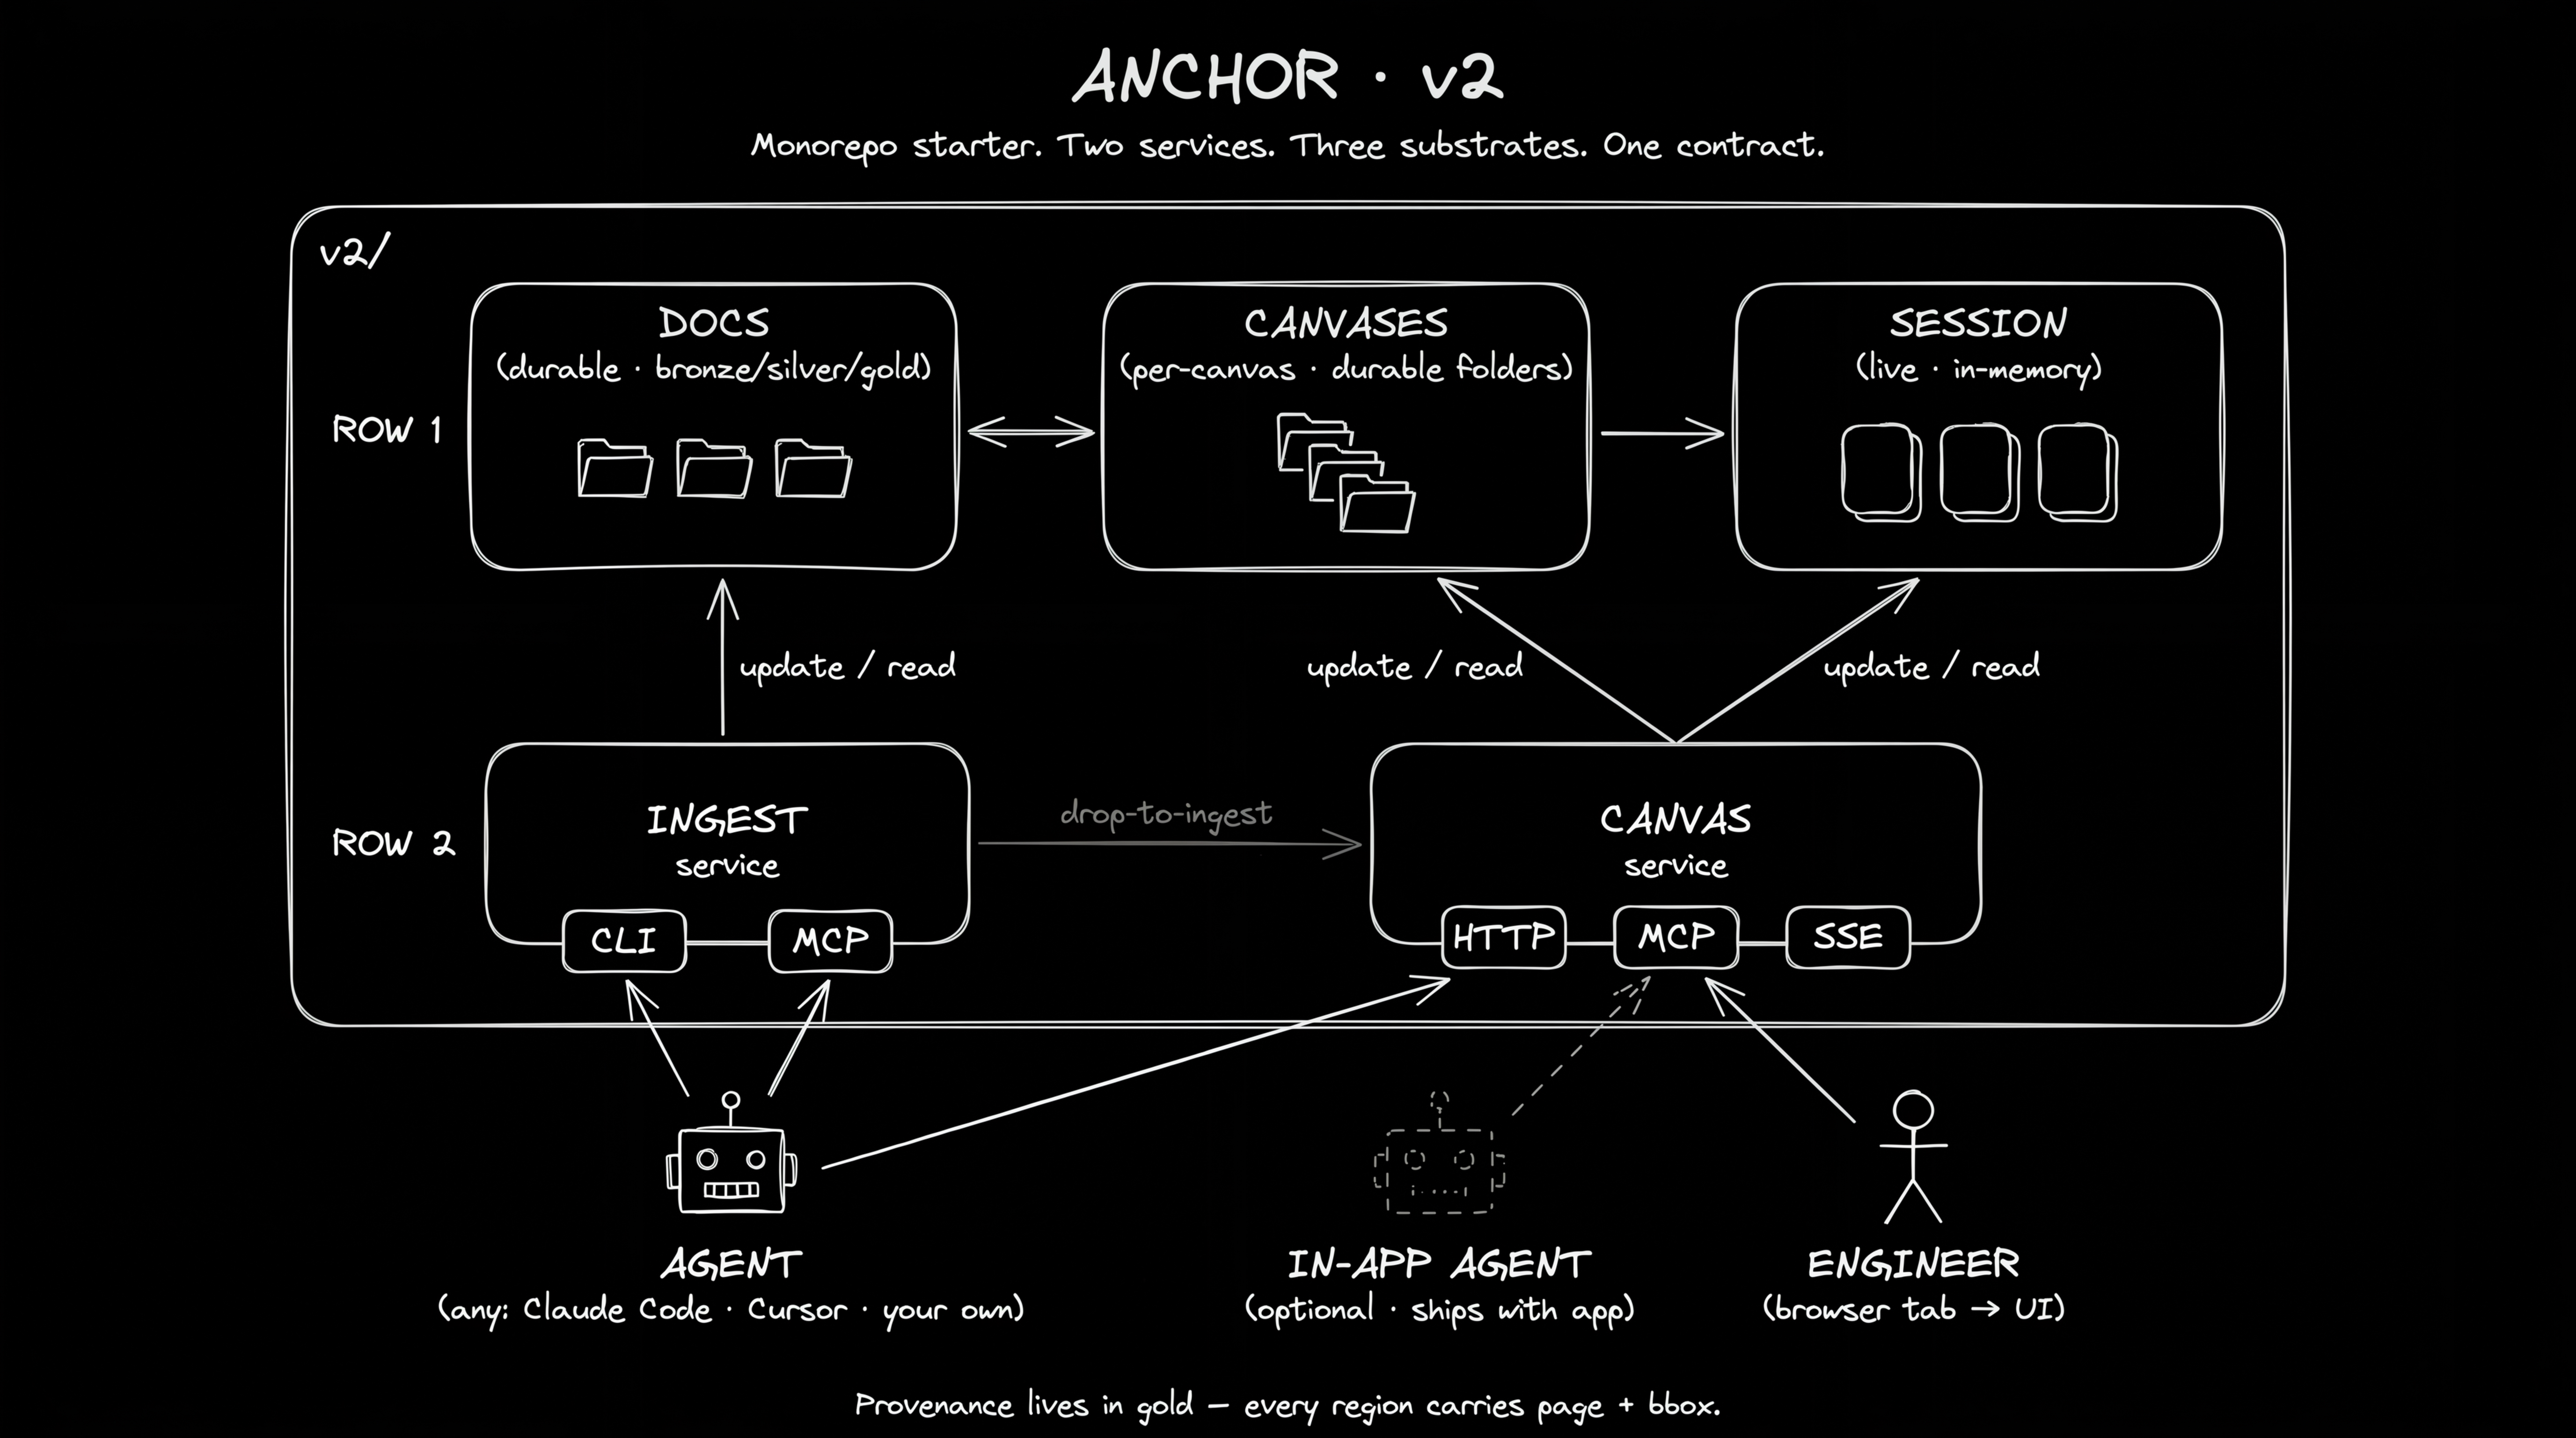
\includegraphics[width=420mm]{architecture-v2-inverted.png}
  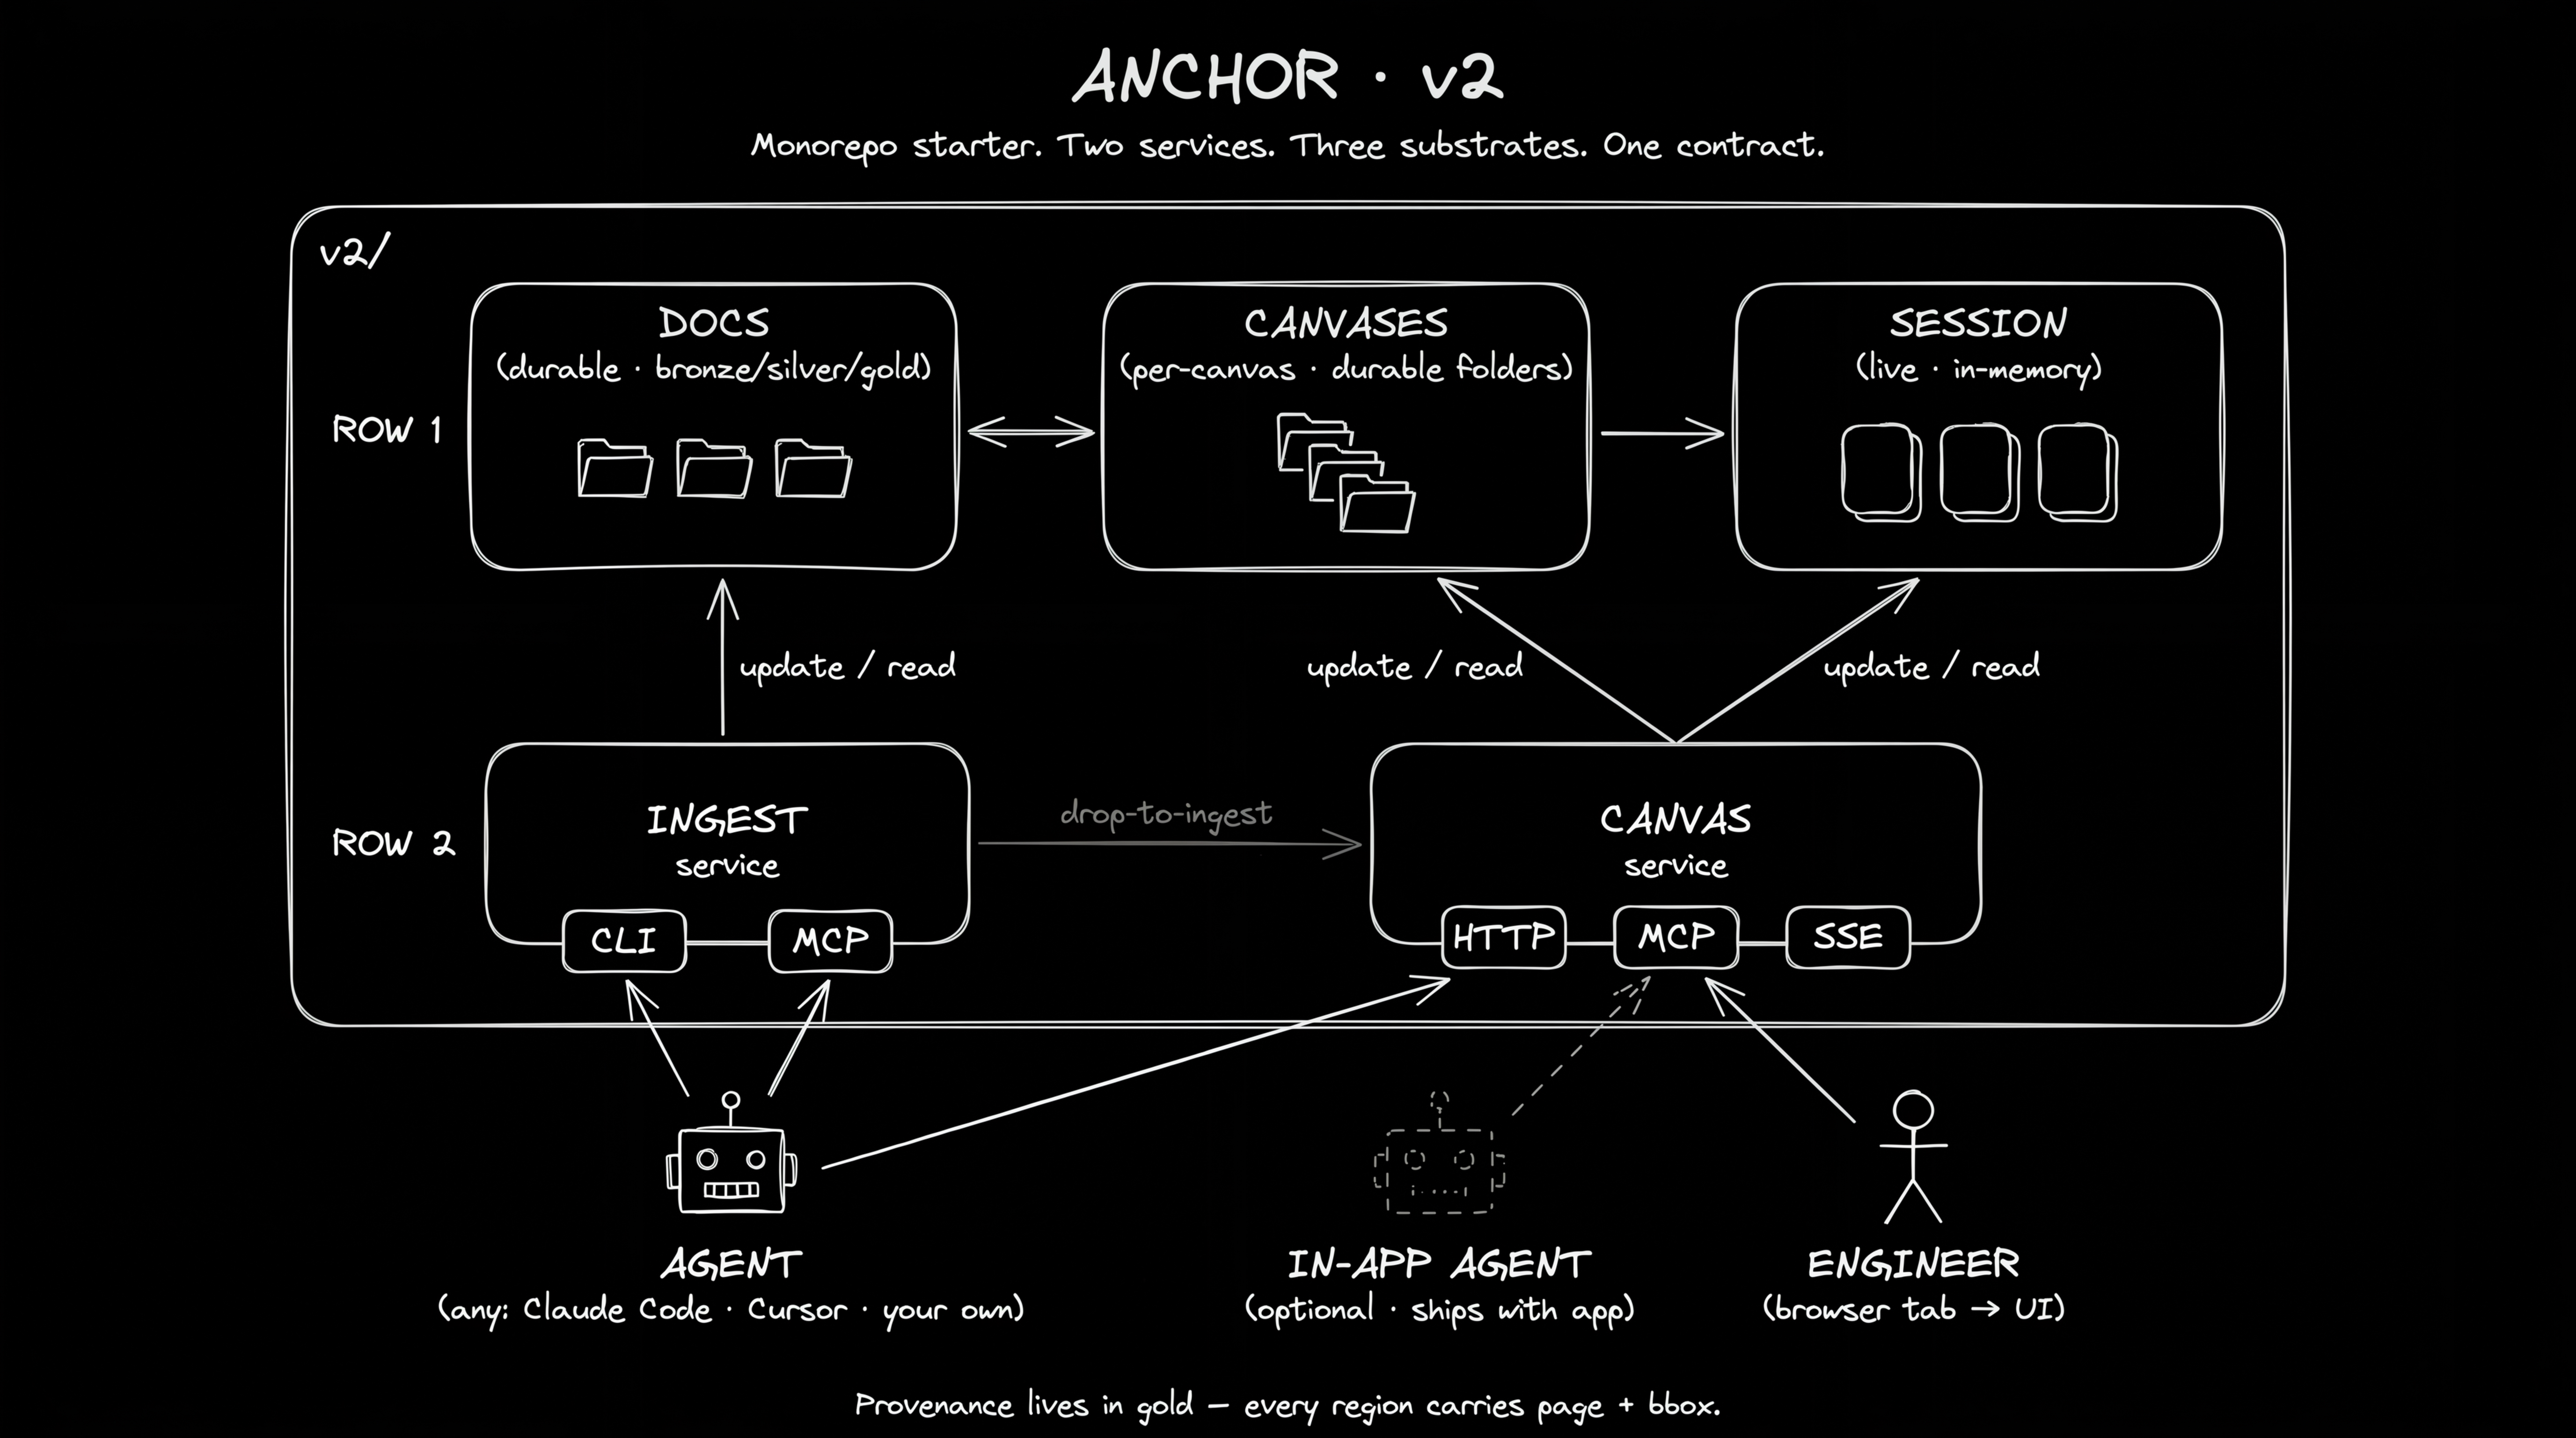
\includegraphics[width=340mm]{architecture-v2-inverted.png}
\end{textblock}

% Funding line at bottom of centre column
% \begin{textblock}{443}(199,556)
\begin{textblock}{443}(199,574)
  \color{centermuted}\centering
  \fontsize{11pt}{14pt}\selectfont
  Funded by Business Finland · Co-Innovation Project Virtual Sea Trial · virtualseatrial.fi\\
  Novia UAS · Åbo Akademi University
\end{textblock}

% ---------------------------------------------------------------------
%  RIGHT COLUMN — graphical abstract + industry value + QR
% ---------------------------------------------------------------------
\begin{textblock}{157}(670,\contentTop)   % rightColX (656) + panelPad (14)
  \color{paneltext}\fontsize{11pt}{15pt}\selectfont\RaggedRight

  \panelhead{The canvas}
  % 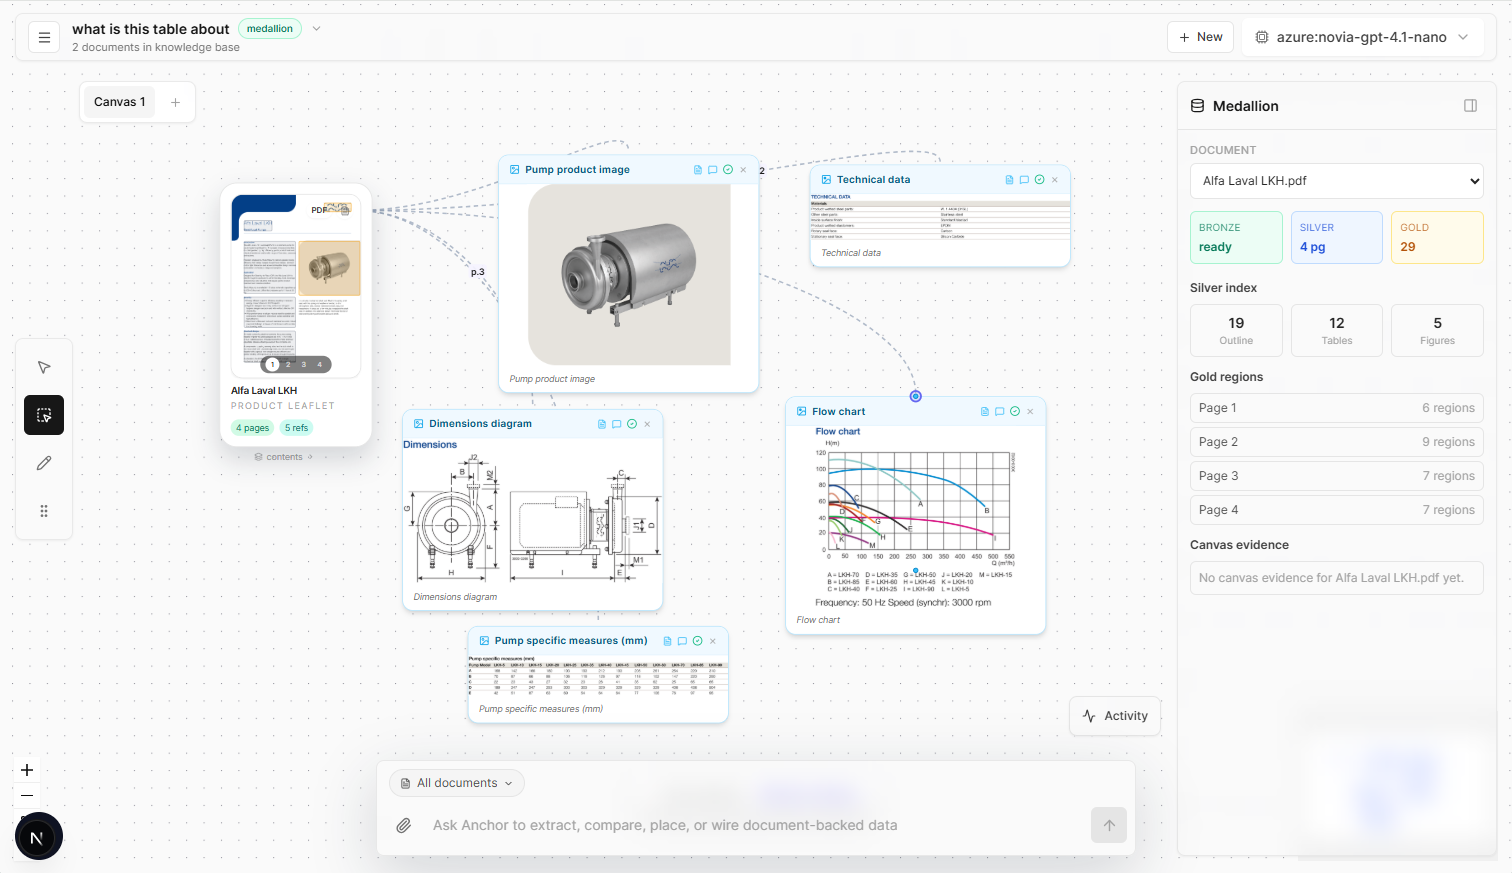
\includegraphics[width=\linewidth]{ui_overview.png}
  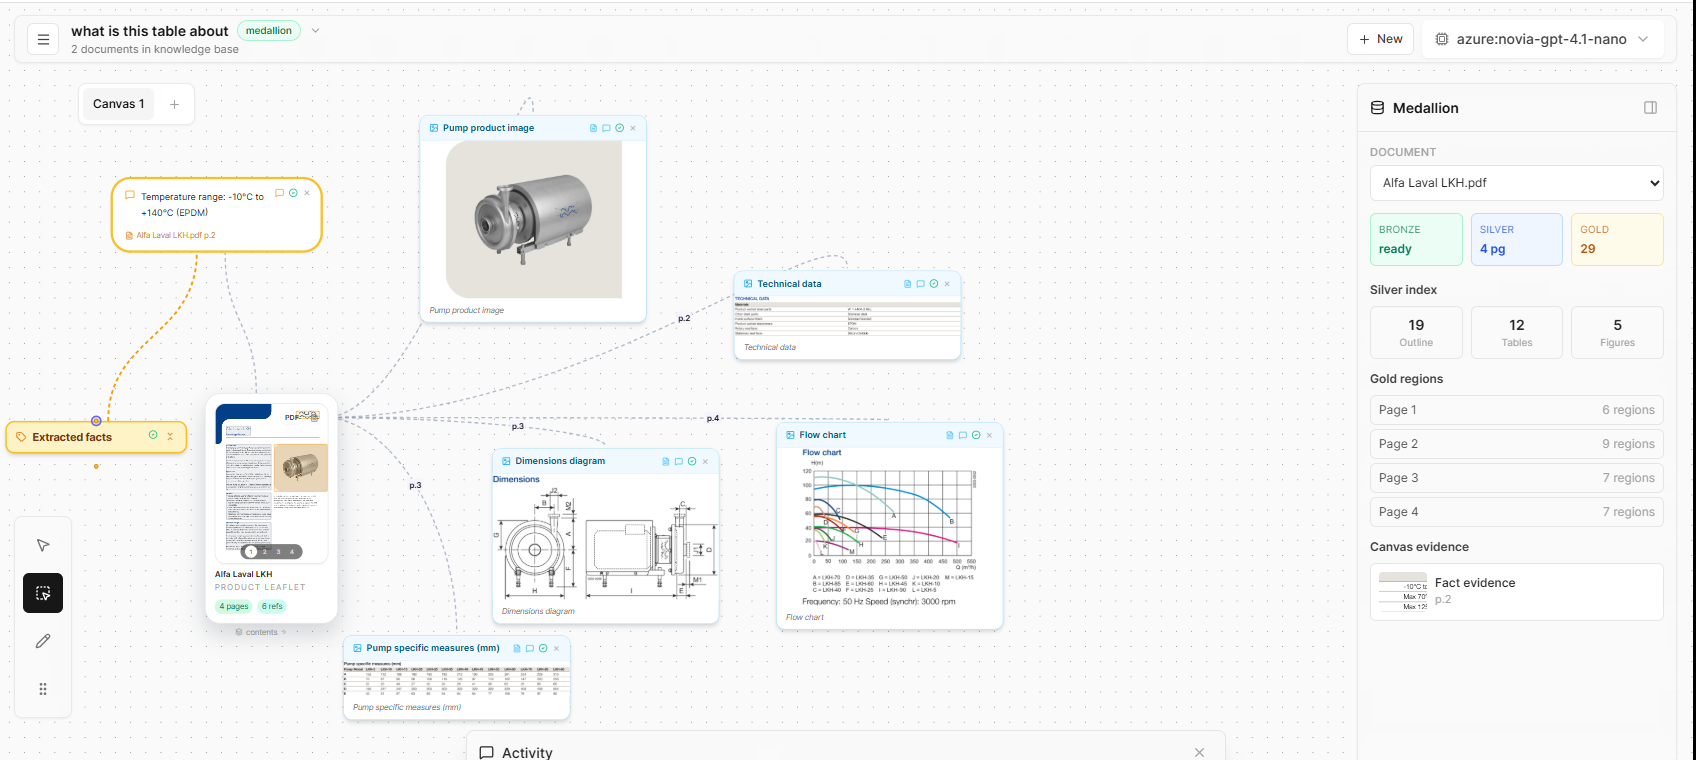
\includegraphics[width=\linewidth]{grounded_canvas.png}
  \vspace{1mm}
  {\fontsize{8.5pt}{11pt}\selectfont\color{panelmuted}
   % Question top. Cards carry source crops with one-click jump to the
   % PDF region. Right rail: bronze\,\arr\,silver\,\arr\,gold ingestion
   % of the active datasheet.
   The canvas shows the proof loop: a grounded answer, its document source,
   PDF-derived visual regions, and the medallion status of the active datasheet.\par}

  \panelhead{Evidence Loop}
  \begin{itemize}\setlength{\itemsep}{1.5pt}\setlength{\parsep}{1pt}\setlength{\leftmargin}{4mm}
    \item Ask a question about a product datasheet.
    \item The agent reads canvas context and document indexes.
    \item The answer becomes a canvas card or table.
    \item The source chip opens the PDF page and bbox behind the claim.
    % \item Repeat.
  \end{itemize}

  \panelhead{Why Industry Should Care}
  \begin{itemize}\setlength{\itemsep}{1.5pt}\setlength{\parsep}{1pt}\setlength{\leftmargin}{4mm}
    \item Fewer copy-paste errors from datasheets into engineering work.
    \item Faster review because source pages are one click away.
    \item Better handoff between engineers, agents, and simulation workflows.
    \item Local-first project data that can be inspected, copied, and versioned.
    \item Works with practical product leaflets, not only clean academic PDFs.
  \end{itemize}

  % \panelhead{Self-hosted}
  \panelhead{Local Demo}
  \begin{itemize}\setlength{\itemsep}{1.5pt}\setlength{\parsep}{1pt}\setlength{\leftmargin}{4mm}
    % \item Runs on a laptop, server, or air-gapped PC. No cloud
    %   account, no telemetry.
    % \item Each canvas is a folder. Copy, share, version-control.
    % \item Open source.
    \item Runs locally with Node.js, Python 3.12, uv, and model credentials.
    \item Current demo uses file-backed documents and conversations; PostgreSQL is not required.
    \item \texttt{git clone} \arr{} \texttt{npm install} \arr{} \texttt{uv sync} \arr{} \texttt{npm run dev}.
  \end{itemize}

  \panelhead{Read more}
  \vspace{1mm}
  \begin{center}
    \qrcode[height=38mm]{https://github.com/Novia-RDI-Seafaring/anchor-kb-ui-RAG}
  \end{center}
  \vspace{1mm}
  {\centering\fontsize{9.5pt}{12pt}\selectfont
   github.com/Novia-RDI-Seafaring/\\anchor-kb-ui-RAG\par}
  \vspace{1mm}
  {\centering\fontsize{8.5pt}{11pt}\selectfont\color{panelmuted}
   Source code and local setup instructions.\par}
  \vspace{2mm}
  \vfill
  {\color{panelmuted}\fontsize{8.5pt}{11pt}\selectfont
   Industry presentation · Vaasa, 2026\par}
\end{textblock}

\end{document}
